\documentclass[a4paper, 12pt]{article}
\usepackage[total={17cm,25cm}, top=2.5cm, left=2.5cm, right=2.5cm,  includefoot]{geometry}
\usepackage[utf8]{inputenc}
\usepackage{array}
\usepackage{multirow}
\usepackage{hhline}
\usepackage{gensymb}
\usepackage{graphicx}
\graphicspath{ {} }
\usepackage[czech]{babel}
\usepackage{enumitem}
\usepackage{pdfpages}
\usepackage{amsmath}
\usepackage{verbatim}
\usepackage{listings}
\usepackage{hyperref}
\usepackage{amssymb}


\pagestyle{empty} % vypne číslování stránek




\usepackage[OT2,OT1]{fontenc}
\newcommand\cyr
{
\renewcommand\rmdefault{wncyr}
\renewcommand\sfdefault{wncyss}
\renewcommand\encodingdefault{OT2}
\normalfont
\selectfont
}
\DeclareTextFontCommand{\textcyr}{\cyr}
\def\cprime{\char"7E }
\def\cdprime{\char"7F }
\def\eoborotnoye{\char’013}
\def\Eoborotnoye{\char’003}


\begin{document}



\begin{titlepage}
\begin{center}
\noindent
\Large \textbf{České vysoké učení technické v Praze }\\ Fakulta stavební
\vspace{5cm}

\huge

%vložení loga cvut
\begin{figure}[h!]
	\centering
	
\includegraphics[width=7cm]{pictures/logo.png}
\end{figure}

\vspace{0.5cm}

Algoritmy v digitální kartografii \\

\vspace{3cm}

\Huge  
Digitální model terénu a jeho analýzy\\

\vspace{2cm}

\Large
Bc. Petra Pasovská \\
Bc. David Zahradník \\

\end{center}

\end{titlepage}




\pagestyle{plain}     % zapne obyčejné číslování
\setcounter{page}{1}  % nastaví čítač stránek znovu od jedné

\tableofcontents
\newpage

\section{Zadání}
Níže uvedené zadání je kopie ze stránek předmětu. 

\begin{figure}[h!]
	\centering
	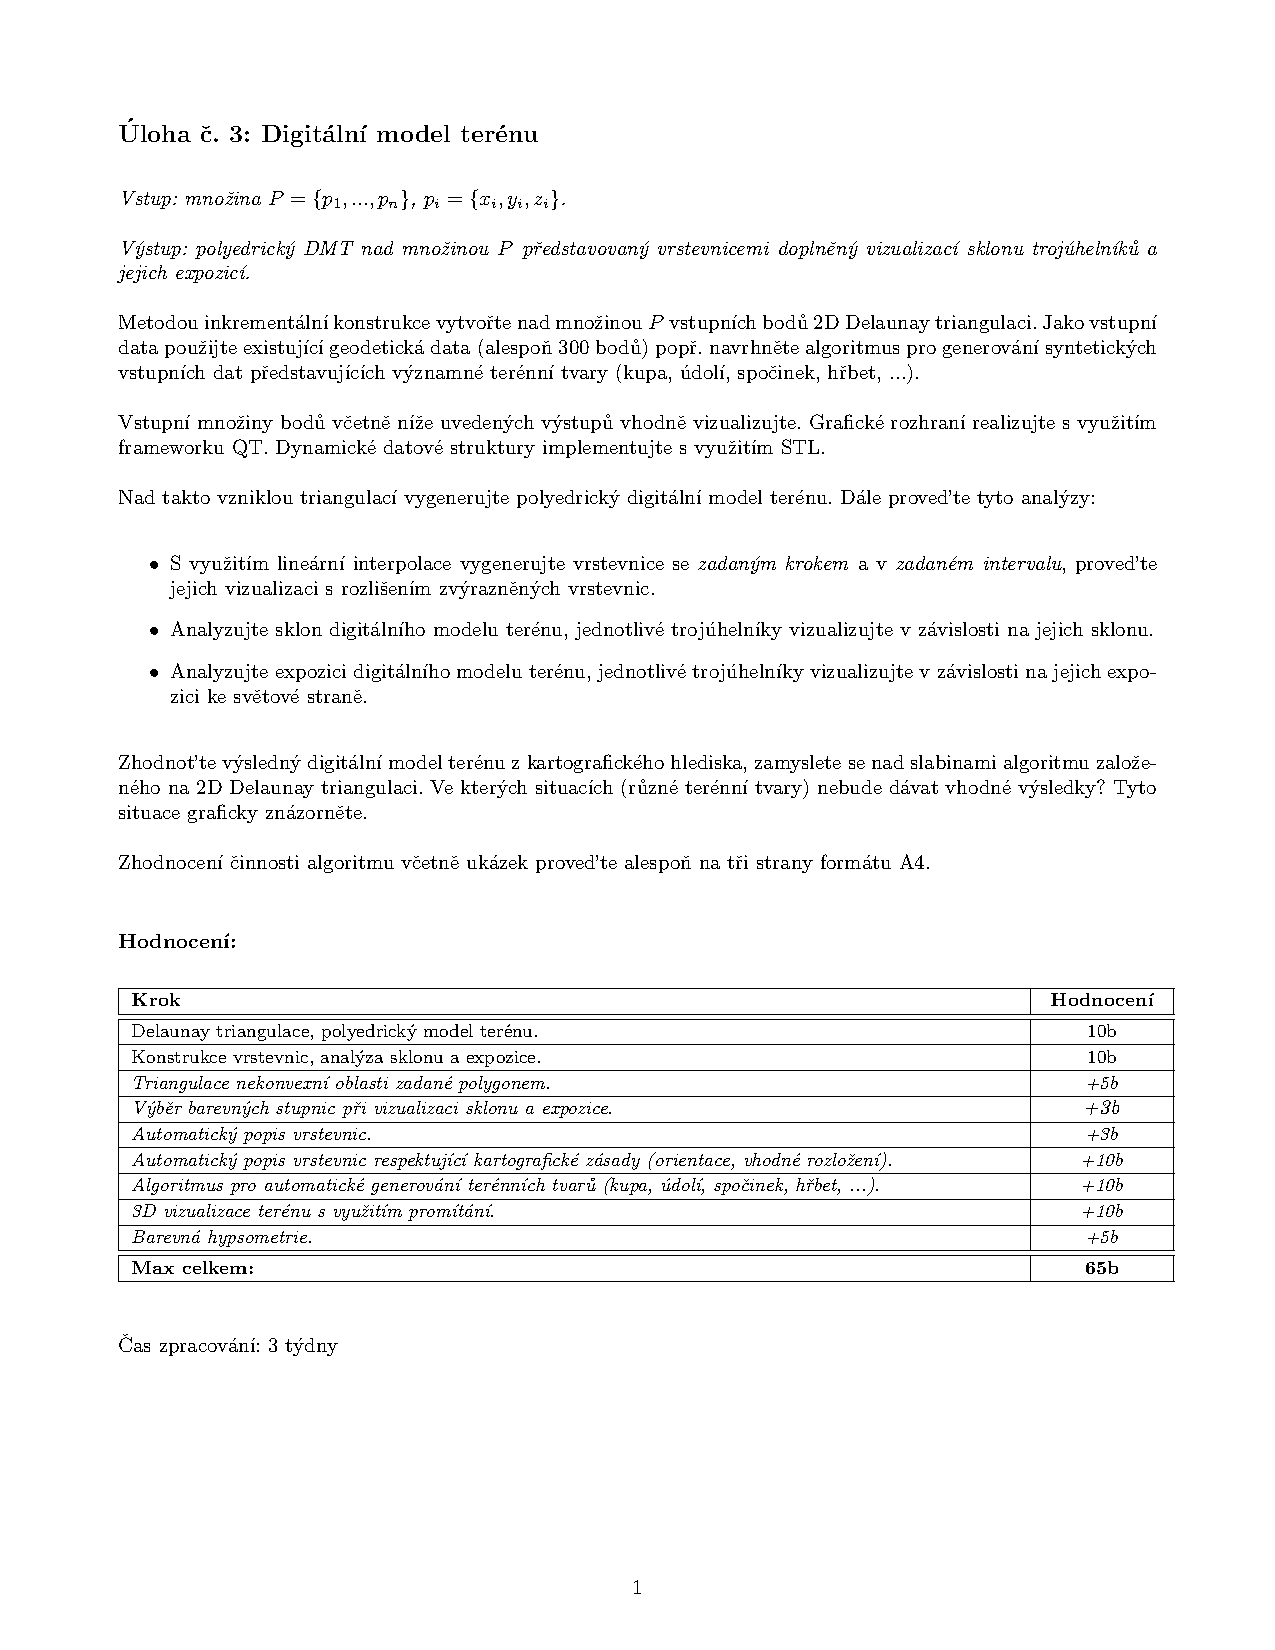
\includegraphics[clip, trim=0cm 5cm 0cm 0cm, width=1.2\textwidth]{zadani.pdf}
\end{figure}

\subsection{Údaje o bonusových úlohách}
Nebyly vytvořeny žádné bonusové úlohy.


\clearpage

\section{Popis a rozbor problému}
Hlavním cílem této úlohy je tvorba aplikace, která nad výškopisnými body vytvoří Delaunay triangulaci, vrstevnice a vypočte sklon a expozici k světovým stranám.\\
\\
Obecně triangulační algoritmy jsou nejvíce zkoumané algoritmy digitální kartografie v dnešní době. Slouží k různým účelům např. tvorba digitálního modelu terénu, plánování pohybu robotů, detekce otisků prstů.  [Zdroj: 1]
\\


\section{Popis použitých algoritmů}
Existuje několik způsobů jak vytvořit triangulaci s různými kritérii. V této úloze jsme ze zabývali Delaunay triangulací pomocí metody inkrementální konstrukce.

\subsection{Delaunay triangulací}
Delaunay triangulace je nejčastěji používanou trianglucí při tvorbě digitálního modelu terénu. Delaunay triagulaci lze provádět v rovině i v prostoru.
\\
\subsubsection{Vlastnosti}
Uvnitř opsané kružnice libovolného trojúhelníku triangulace neleží žádný jiný bod.
\\
Maximalizuje minimální úhel, avšak neminimalizuje maximální úhle v trojúhelníku.
\\
Vůči kritériu minimálního úhlu je lokálně i globálně optimální.
\\
Triangulace je jednoznačná pokud čtyři body neleží na kružnici.
\\

Triangulace byla realizována pomocí metody inkrementální konstrukce. Tento algoritmus je založen na postupném hledání bodu, který k bodům hrany tvoří minimální opsanou kružnici. Každá hrana je orientovaná a bod se hledá pouze v její levé polorovině.\\
Je-li nalezen bod s výše uvedeným kritériem vytvoří se dvě nové hrany, které jsou přidány do triangulace. Nenalezne-li se daný bod, prohodí se orientace hrany a hledání pokračuje.\\
Hrany, které nebyly zlegalizovány (nebyl k ní ještě nalezen třetí bod), jsou ukládány do struktury Active Edge List (AEL). Pokud k dané hraně byl nalezen tří bod, hrana se ze struktury odstraní. Než je hrana vložena do struktury, kontroluje se zda hrana už ve struktuře není s opačnou orientací, pokud je, hrana se nevloží. Algoritmus běží dokud struktura AEL není prázdná.

\subsubsection{Implementace metody}
\begin{enumerate}
\item Nalezení pivota q a k němu nejbližší bod:  $ q = min(y_i) $ 
\item Hledání prvního Delaunay bodu.
\item Vytvoření prvního Delaunay trojúhelníku.
\item Hrany trojúhelníka se uloží do triangulace a do AEL.
\item Dokud není AEL prázdný proveď.
\subitem Hledej Delaunay bod k hraně z AEL.
\subitem Pokud Delaunay bod existuje.
\subsubitem Přidej nové hrany do DT.
\subsubitem Pokud nová hrana není v AEL přidej.
\end{enumerate}

\subsection{Vrstevnice}
V úloze byly vrstevnice konstruovány lineární interpolací. U lineární interpolace je rozestup vrstevnice mezi dvěma body konstantní, tedy i spád. Při konstrukci vrstevnic hledáme průsečnici vodorovné roviny o výšce Z a rovinu trojúhelníka triangulace.\\

\subsubsection{Implementace metody}
\begin{enumerate}
\item Pro všechny hrany triangulace:
\subitem Otestuj zda hrana protíná vodorovnou rovinu o výšce Z:
\subitem Pokud protíná spočti polohové souřadnice.
\subitem Vytvoř hranu tvořící vrstevnici.

\end{enumerate}

\subsection{Sklon terénu}
Skon terénu je definován jako úhle mezi normálovým vektorem (0,0,1) a normálovým vektorem roviny trojúhelníku.

\subsubsection{Implementace metody}
\begin{enumerate}
\item Pro všechny trojúhelníky triangulace:
\subitem Vypočti sklon:
\end{enumerate}

\subsection{Expozice terénu}
Expozice terénu je definována jako azimut k průmětu normálového vektoru roviny trojúhelníka do roviny x,y.

\subsubsection{Implementace metody}
\begin{enumerate}
\item Pro všechny trojúhelníky triangulace:
\subitem Vypočti expozici:
\end{enumerate}

\section{Informace o bonusových úlohách}


\section{Vstupní data}


\section{Výstupní data}



\clearpage

\section{Dokumentace}
\subsection{Třídy}
\subsubsection{Algorithms}
Třída Algorithms obsahuje několik metod. Metody jsou určeny pro výpočty použitých algoritmů.
\\

\textbf{double distance(QPoint3D p1, QPoint3D p2)}\\
Metoda, jejíž návratová hodnota je typu double, vrací velikost spojnice mezi dvěma body.
\\

\textbf{TPosition getPointLinePosition(QPoint \&q, QPoint \&a, QPoint \&b)}\\
Tato metoda slouží k určení pozice bodu q vůči linii tvořené body a, b. Výstupem metody je LEFT, RIGHT nebo ON.\\

\textbf{double getCircleRadius(QPoint3D \&p1, QPoint3D \&p2, QPoint3D \&p3, QPoint3D \&c)}\\
Metoda jejíž návratová hodnota je typu double, vrací velikost poloměru kružnice tvořené třemi vstupními body.\\

\textbf{int getNearestPoint(QPoint3D \&p, std::vector<QPoint3D> \&points)}\\
Tato metoda slouží k nalezení indexu nejbližšího bodu k bodu p.\\

\textbf{int getDelaunayPoint(QPoint3D \&s, QPoint3D \&e, std::vector<QPoint3D> \&points)}\\
Tato metoda slouží k nalezení indexu bodu, který splňuje Delaunay vlastnosti.\\

\textbf{std::vector<Edge> DT(std::vector<QPoint3D> \&points)}\\
Metoda vytváří nad vektorem bodů Delaunay triangulaci, které se reprezentuje jako vektor hran.\\

\textbf{QPoint3D getContourPoint(QPoint3D \&p1, QPoint3D \&p2, double z)}\\
Metoda vypočte průsečík hrany, tvořenou 3D body p1 a p2, a rovinou definovanou z souřadnicí.\\

\textbf{std::vector<Edge> createContours(std::vector<Edge> \&dt, $double z_min, double z_max, double dz$)}\\
Metoda z triangulace dt v zadaném intervalu v ose Z $<z_min ; z_max>$ s intervalem vrstevnic dz vrátí vektor hran definující vrstevnice.\\

\textbf{double getSlope(QPoint3D \&p1, QPoint3D \&p2, QPoint3D \&p3)}\\
Tato metoda slouží k vypočetní hodnoty sklonu trojúhelníku definovanému 3D body p1, p2 a p3.\\

\textbf{double getAspect(QPoint3D \&p1, QPoint3D \&p2, QPoint3D \&p3)}\\
Tato metoda slouží k vypočetní hodnoty expozice trojúhelníku definovanému 3D body p1, p2 a p3.\\

\textbf{std::vector<Triangle> analyzeDTM(std::vector<Edge> \&dt)}\\
\\

\textbf{std::vector<QPoint3D> generateHill()}\\
\\

\textbf{std::vector<QPoint3D> generateValley())}\\
\\

\textbf{std::vector<QPoint3D> generateMountains()}\\
\\

\textbf{std::vector<QPoint3D> generateRest())}\\
\\

\subsubsection{Draw}
Třída Draw obsahuje několik metod. Metody jsou určeny pro generování a vykreslování proměných.
\\

\textbf{void paintEvent(QPaintEvent *e)}\\
Metoda slouží k vykreslení vytvořených, generovaných bodů a zobrazení výsledků použitých algoritmů.
\\

\textbf{void mousePressEvent(QMouseEvent *e)}\\
Metoda uloží bod se souřadnicemi místa kliknutí v zobrazovacím okně.
\\

\textbf{void clearDT()}\\
Metoda slouží k vymazání proměnných a k překreslení
\\

\textbf{void clearPoints()}\\
Metoda slouží k vymazání bodů.
\\

\textbf{void setPoints(std::vector<QPoint3D> points\_)}\\
Metoda slouží pro převod bodů do vykreslovacího okna.\\

\textbf{std::vector<QPoint3D> \& getPoints()}\\
Metoda slouží pro převod bodů z vykreslovacího okna.\\

\textbf{std::vector<Edge> \& getDT()}\\
Metoda slouží pro převod Delaunay triangulace z vykreslovacího okna.\\

\textbf{void setDT(std::vector<Edge>\&dt\_)}\\
Metoda slouží pro převod Delaunay triangulace do vykreslovacího okna.\\

\textbf{void setContours(std::vector<Edge>\&contours\_)}\\
Metoda slouží pro převod vrtevnic do vykreslovacího okna.\\

\textbf{void setDTM(std::vector<Triangle> \&dtm\_)}\\
\\

\subsubsection{SortByXAsc}
Třída SortByXAsc slouží k porovnání souřadnic v ose x.\\


\textbf{bool operator()(QPoint \&p1, QPoint \&p2)}\\
Přetížený operátor () vrátí bod s větší souřadnicí x z dvojice bodů.\\

\subsubsection{Edge}
\textbf{Edge(QPoint3D \&start, QPoint3D \&end)}\\
Třída Edge je konstruována ze dvou 3D bodů, počátek a konec hrany. Třída slouží k uložení hrany triangulace a nebo vrstevnic.\\
    
\textbf{QPoint3D \&getS()}\\
Metoda vrátí počáteční bod hrany.\\

\textbf{QPoint3D \& getE()}\\
Metoda vrátí koncový bod hrany.\\

\textbf{void switchOr()}\\
Metoda prohodí orientaci hrany.\\

\subsubsection{QPoint3D}
\textbf{QPoint3D(double x, double y, double z\_)}\\
Třída QPoint3D je odvozena z třídy QPointF a složí k uložení bodu s informací o výšce.\\

\textbf{double getZ()}\\
Metoda vrátí výšce bodu.\\

\textbf{void setZ(double z\_)}\\
Metoda nastaví výšku bodu.\\

\subsubsection{Triangle}
\textbf{Triangle(QPoint3D \&p1\_, QPoint3D \&p2\_, QPoint3D \&p3\_, double slope\_, double aspect\_))}\\
Třída QPoint3D složí k uložení trojúhelníku definovaného boy p1, p2, p3 a jeho informaci o sklonu a expozici.\\

\textbf{ QPoint3D getP1()}\\
Metoda vrátí první bod trojúhelníku.\\

\textbf{ QPoint3D getP2()}\\
Metoda vrátí druhý bod trojúhelníku.\\

\textbf{ QPoint3D getP3()}\\
Metoda vrátí třetí bod trojúhelníku.\\

\textbf{double getSlope()}\\
Metoda vrátí sklon trojúhelníku.\\

\textbf{double getAspect()}\\
Metoda vrátí expozici trojúhelníku.\\

\subsubsection{Widget}

\textbf{void on\_pushButton\_clicked()}\\
Při stisknutí tlačítka Denaulay se zavolá metoda třídy Algorithms DT a výsledek se zobrazí v okně.
\\

\textbf{void on\_pushButton\_3\_clicked()}\\
Při stisknutí tlačítka Clear se zavolá metoda třídy Draw clearDT.
\\

\textbf{void on\_pushButton\_2\_clicked()}\\
Při stisknutí tlačítka Create Contours se zavolá metoda třídy Algorithms createContours a výsledek se zobrazí v okně.
\\

\textbf{void on\_pushButton\_4\_clicked()}\\
Při stisknutí tlačítka AnalyzeDTM se zavolá metoda třídy Algorithms analyzeDTM a výsledek se zobrazí v okně.
\\

\textbf{void on\_pushButton\_5\_clicked()}\\
Při stisknutí tlačítka Generate a výběru z comboboxu se vygenerují body terénu.
\\



\clearpage
\section{Závěr}
Byla vytvořena aplikace, které nad importovanými body vytvoří Delaunay triangulaci, vykreslí vrstevnice, sklon a expozici terénu. Aplikace má nějaké nedostatky, které autoři nestihli opravit.\\

\subsection{Delaunay triangulce}
Vzhledem implementace triangulace, výběr trojúhelníku z vyhledávání nejmenší opsané kružnice, algoritmus selhává, když body jsou v mřížce. Triangulace je pro tyto body nejednoznačná a další výpočty selhávají.\\

V aplikaci nezle nadefinovat povinné hrany, které jsou důležité pro terénní tvary, jako terénní hrana a propast. Proto algoritmus není použitelný pro data s těmito typy terénní tvarů. Důvod je zřejmý z implementace triangulace.\\

V aplikaci též nelze nastavit zájmovou oblast, proto je nutné před výpočtem algoritmu odstranit body, nad kterými nechceme provádět triangulaci.\\

Aplikace je užitečná pro výškopisná data v terénu bez povinných hran a kde data nepotřebují být upravována, viz předchozí odstavec. \\

\subsection{Vrstevnice}
Pro vykreslení vrstevnic byla použitá lineární interpolace, která má svoje úskalí. Jelikož pro výpočet vrstevnic není řešené vyhlazení vrstevnic, výsledek není vhodný ke chlubení.\\

Autoři neřešili vykreslení hlavní vrstevnice zesílenou čárou ani popis vrstevnic. \\

\subsection{Sklon a expozice terénu}
Při výpočtu sklonu a expozice terénu vzniká problém v rovinatém území. Při výpočtu vznikají zaokrouhlovací chyby, které se promítnou do sklonu a expozice. Proto se terén jeví uživateli nerovinný.\\

Do aplikace by se hodila legenda expozice terénu.\\

\section{Náměty na vylepšení}



\clearpage
\section{Reference}

\begin{enumerate}
\item  BAYER, Tomáš. Geometrické vyhledávání [online][cit. 1. 12.2018]. \\
Dostupné z: https://web.natur.cuni.cz/~bayertom/images/courses/Adk/adk5.pdf  \\




\end{enumerate}
\end{document}



 